%------------------------------------------------
%
% Master.tex
%
% This file contains all the directive to include
% the different part of the document and build it
% during the compilation phase.
%
% To compile correctly the entire document follow
% these commands in a shell positioned in the folder
% that contains the master document (Master.tex):
%
%	1) pdflatex Frontespiece/Frontespiece
%	2) pdflatex Frontespiece/Frontespiece-frn
%	3) pdflatex Frontespiece/Frontespiece
%	4) pdflatex Master
%   5) makeglossaries Master
%	6) pdflatex Master
%	7) pdflatex Master
%------------------------------------------------
%------------------------------------------------
%
% Preamble.tex
%
% This file contains all the settings for a correct
% compilation of the document. Include this file
% before starting the document section.
%------------------------------------------------
\documentclass[paper=A4, fontsize=11pt, parskip=full]{scrreprt}

\usepackage{acronym}
\usepackage{fourier}
\usepackage{graphicx}
\usepackage{ifthen}
\usepackage{lastpage}
\usepackage{longtable}
\usepackage{pdfpages}
\usepackage{sectsty}
\usepackage{siunitx}
\usepackage[utf8]{inputenc}
\usepackage[babel]{csquotes}
\usepackage[T1]{fontenc}
\usepackage[hidelinks]{hyperref}
\usepackage[english, italian]{babel}
\usepackage[nonumberlist, toc]{glossaries}
\usepackage[protrusion=true, expansion=true]{microtype}
\usepackage[automark, headsepline, footsepline, markuppercase]{scrpage2}

\allsectionsfont{\centering \normalfont\scshape}

\pagestyle{scrheadings}

\lehead{Amministrazione di Sistema}
\rohead{Service Desk}
\chead{}
\cfoot{\thepage{} di \pageref{LastPage}}

\setglossarystyle{altlist}
\makeglossaries

\newcommand{\english}[1]{\foreignlanguage{english}{\textit{#1}}}
\newcommand{\keyword}[1]{\textbf{#1}}
\newcommand{\entity}{Ospedale Gaetano Pini}
\newcommand{\printListOfContents}[1]{\ifthenelse{\equal{#1}{TRUE}}{\tableofcontents{}}{}}
\newcommand{\printListOfFigures}[1]{\ifthenelse{\equal{#1}{TRUE}}{\listoffigures{}}{}}
\newcommand{\printListOfTables}[1]{\ifthenelse{\equal{#1}{TRUE}}{\listoftables{}}{}}
\newcommand{\printGlossary}[1]{\ifthenelse{\equal{#1}{TRUE}}{\printglossary[title=Glossario]{}}{}}
\newcommand{\glossarySingolarTerm}[1]{\underline{\gls{#1}}}
\newcommand{\glossaryPluralTerm}[1]{\underline{\glspl{#1}}}
\newcommand{\attribute}[1]{\textsc{#1}}

%------------------------------------------------
%
% AcronymDatabase.tex
%
% This file contains the database of the acronym
% used in the document. Include it in the preable
% before starting the document.
%------------------------------------------------
\acrodef{Access-Management}[AM]{\english{Access Management}}
\acrodef{Active-Directory}[AD]{\english{Active Directory}}
\acrodef{Asset-Management}[AM]{\english{Asset Management}}
\acrodef{Assistant-Service-Request}[ASR]{Assistant Service Request}
\acrodef{Availability-Management}[AM]{\english{Availability Management}}

\acrodef{Centro-Elaborazione-Dati}[CED]{Centro Elaborazione Dati}
\acrodef{Change-Advisory-Board}[CAB]{\english{Change Advisory Board}}
\acrodef{Configuration-Item}[CI]{\english{Configuration Item}}
\acrodef{Change-Management}[CM]{\english{Change Management}}
\acrodef{Capacity-Management}[CM]{\english{Capacity Management}}
\acrodef{Configuration-Management}[CM]{\english{Configuration Management}}
\acrodef{Configuration-Management-DataBase}[CMDB]{\english{Configuration Management DataBase}}
\acrodef{Configuration-Management-System}[CMS]{\english{Configuration Management System}}
\acrodef{Configuration-Record}[CR]{\english{Configuration Record}}
\acrodef{Content-Management-System}[CMS]{\english{Content Management System}}

\acrodef{DataBase-Management-System}[DBMS]{\english{DataBase Management System}}
\acrodef{Distribuited-File-System}[DFS]{Distribuited File System}

\acrodef{Enhancement-Change-Request}[ECR]{\english{Enhancement Change Request}}
\acrodef{Event-Management}[EM]{\english{Event Management}}

\acrodef{First-In-First-Out}[FIFO]{\english{First In First Out}}
\acrodef{Forward-Schedule-Change}[FSC]{\english{Forward Schedule of Change}}

\acrodef{Human-Resources}[HR]{\english{Human Resources}}

\acrodef{Incident-Management}[IM]{\english{Incident Management}}
\acrodef{Information-Technology}[IT]{\english{Information Technology}}
\acrodef{Information-Technology-Infrastructure-Library}[ITIL]{\english{Information Technology Infrastructure Library}}
\acrodef{Internet-Service-Provider}[ISP]{\english{Internet Service Provider}}

\acrodef{Knowledge-Base}[KB]{\english{Knowledge Base}}
\acrodef{Known-Error-DataBase}[KEDB]{\english{Known Error DataBase}}

\acrodef{Operational-Level-Agreement}[OLA]{\english{Operational Level Agreement}}

\acrodef{Personal-Computer}[PC]{\english{Personal Computer}}
\acrodef{Problem-Management}[PM]{\english{Problem Management}}
\acrodef{Plan-Do-Check-Act}[PDCA]{\english{Plan Do Check Act}}

\acrodef{Request-Fulfillment}[RF]{\english{Request Fulfillment}}
\acrodef{Request-For-Change}[RFC]{\english{Request For Change}}

\acrodef{Software-as-a-Service}[SaaS]{\english{Software as a Service}}
\acrodef{Service-Continuty-Management}[SCM]{\english{Service Continuty Management}}
\acrodef{Service-Level-Agreement}[SLA]{\english{Service Level Agreement}}
\acrodef{Service-Level-Management}[SLM]{\english{Service Level Management}}
\acrodef{Service-Level-Requirements}[SLR]{\english{Service Level Requirements}}
\acrodef{Service-Point-Of-Contact}[SPOC]{\english{Service Point Of Contact}}

\acrodef{Uninterruptible-Power-Supply}[UPS]{\english{Uninterruptible Power Supply}}

%------------------------------------------------
%
% GlossaryDatabase.tex
%
% This file contains the terms that are present
% in the glossary of the document.
%------------------------------------------------
\newglossaryentry{efficace}
{
	name		= {efficace},
	plural		= {efficaci},
	description = {Un servizio che produce pienamente l'effetto richiesto o desiderato}
}

\newglossaryentry{efficiente}
{
	name		= {efficiente},
	plural		= {efficienti},
	description = {Raggiungimento dell'obiettivo preposto nel modo migliore possibile ossia usando al meglio le risorse a propria disposizione}
}

\newglossaryentry{framework}
{
	name		= {framework},
	plural		= {frameworks},
	description = {In informatica, specialmente nello sviluppo \english{software}, è un'architettura logica di supporto su cui un \english{software}/servizio può essere progettato e realizzato spesso facilitandone lo sviluppo}
}

\newglossaryentry{incidente}
{
	name		= {incidente},
	plural		= {incidenti},
	description	= {Un incidente (\english{incident}) è un qualsiasi evento che non fa parte dell'operatività \english{standard} del servizio e che causa una riduzione o un'interruzione del servizio offerto}
}

\newglossaryentry{overflow}
{
	name		= {overflow},
	plural		= {overflow},
	description = {Condizione che accade quando un calcolo produce un risultato che è più grande di quello che può essere memorizzato}
}

\newglossaryentry{release}
{
	name		= {release},
	plural		= {releases},
	description = {Nell'ambito dello sviluppo di un servizio una \english{release} è una specifica versione dello stesso resa disponibile agli utenti finali. E' univocamente identificata in modo che sia possibile distinguerla dalle precedenti. Convenzionalmente si suddividono in \english{release} maggiori (\english{Major Release}) quando le differenze dalla precedente versione riguardano sostanziali evoluzioni delle funzionalità offerte e \english{release} minori (\english{Minor Release}) quando le differenze riguardano principalmente correzioni di malfunzionamenti}
}

\newglossaryentry{rollout}
{
	name		= {roll out},
	plural		= {roll out},
	description = {Nel campo dei sistemi informativi il termine \english{roll out} è comunemente impiegato per identificare il processo con cui un servizio viene attivato a partire da una istanza iniziale. Durante il \english{roll out} del servizio si trovano le fasi progettuali di \english{training}, di collaudo e di messa in esercizio}
}

\newglossaryentry{workaround}
{
	name		= {workaround},
	plural		= {workarounds},
	description	= {Si tratta di una correzione temporanea ad un incidente oppure una sequenza di azioni alternative a quella che produce l'incidente che però rende utilizzabile, anche se in versione ridotta, il servizio}
}

\begin{document}

\includepdf[pages={1}]{Frontespiece/Frontespiece.pdf}

\clearpage

\printListOfContents{TRUE}

\printListOfTables{TRUE}

\printListOfFigures{TRUE}

%------------------------------------------------
%
% Abstract.tex 
%
% This section introduce the document.
%------------------------------------------------
\chapter[Abstract]{abstract}
\label{abs}
All'interno di una realtà aziendale complessa, come l'ente oggetto di questo capitolato, è doveroso istituire ed istruire dei processi e delle funzioni di controllo che mirano a garantire che i servizi offerti agli utenti siano il più \keyword{efficaci} ed \keyword{efficienti} possibile.

Un possibile metodo per ottenere degli ottimi livelli di servizi offerti e allo stesso tempo avere un \keyword{miglioramento permanente e continuo}, degli stessi, consiste nell'adottare un \english{\glossarySingolarTerm{framework}} quale, per esempio, \ac{ITIL} per la gestione del proprio dipartimento \acs{IT}.

Lo scopo che questo documento si prefigge di raggiungere consiste nella progettazione e la conseguente implementazione di una particolare funzionalità presente nel \english{framework}, la funzionalità di \keyword{\english{Service Desk}}. Verranno inoltre illustrati alcuni dei processi, che direttamente, ha lo scopo di amministrare.

Essi sono: 

\begin{itemize}
\item{\acf{EM}}
\item{\acf{IM}}
\item{\acf{RF}}
\end{itemize}

%------------------------------------------------
%
% Structure.tex 
%
% This section describe the structure of the
% document.
%------------------------------------------------
\section[Struttura del documento]{struttura del documento}
\label{abs-document-structure}
Il seguente documento è stato suddiviso nei seguenti capitoli:

\begin{itemize}
\item{\keyword{Capitolo 1}: funzionalità di \english{Service Desk}}
\item{\keyword{Capitolo 2}: definizione dei processi}
\item{\keyword{Capitolo 3}: \ac{Service-Level-Requirements} della funzione di \english{Service Desk}}
\item{\keyword{Capitolo 4}: \ac{Service-Level-Agreement} della funzione di \english{Service Desk}}
\item{\keyword{Capitolo 5}: piano di \english{roll out} del nuovo \english{Service Desk}}
\end{itemize}

%------------------------------------------------
%
% Recipient.tex 
%
% This section show the recipient of this
% document.
%------------------------------------------------
\section{A chi è rivolto}
\label{abs-recipient}
Il presente documento è rivolto ai membri del consiglio di amministrazione dell'Ospedale Gaetano Pini di Milano. Alla C.A. dei dottori:

\begin{itemize}
\item{Dott. Amedeo Tropiano -- Direttore Generale}
\item{Dott.ssa Loredana Maspes -- Direttore Amministrativo}
\item{Dott. Nunzio Angelo Buccino -- Direttore Sanitario}
\end{itemize}

%------------------------------------------------
%
% Hightlighting.tex 
%
% This section describe the hightlightining
% used in the document.
%------------------------------------------------
\section[Convenzioni tipografiche]{convenzioni tipografiche}
\label{abs-hightlighting}
Nel seguente documento si sono introdotte le seguenti convenzioni tipografiche al fine di consentire una lettura scorrevole dello stesso.

Esse sono:

\begin{itemize}
\item{\textbf{grassetto} per evidenziare i termini più importanti presenti nel paragrafo;}
\item{\textit{corsivo} per evidenziare i termini in lingua inglese;}
\item{\underline{sottolineato} per la prima occorrenza di termini presenti nel glossario finale.}
\end{itemize}

%------------------------------------------------
%
% ServiceDesk.tex 
%
% This section introduces the service desk
% function.
%------------------------------------------------
\chapter[Funzione di Service Desk]{funzione di service desk}
\label{sd}

%------------------------------------------------
%
% Introduction.tex 
%
% This section introduces the incident management
% process.
%------------------------------------------------
\section[Introduzione]{introduzione}
\label{im-introduction}
Questo capitolo descrive il processo di \acf{Incident-Management} per la funzione di \english{Service Desk} dell'\entity{}.

Il processo fornisce un metodo coerente che gli utenti devono seguire in caso di disservizi durante la normale operatività all'interno dell'\entity{}.

\subsection[Scopo principale]{scopo principale}
\label{im-introduction-scope}
Lo scopo principale del processo di \ac{Incident-Management} è quello di \keyword{ripristinare il funzionamento normale dei servizi il più rapidamente possibile} e \keyword{ridurre al minimo l'impatto negativo} sulle operazioni di \english{business}, garantendo così che i migliori livelli possibili di \keyword{qualità del servizio} e \keyword{disponibilità} siano mantenuti.

\attribute{nota}: attraverso la dicitura ``normale funzionamento del servizio'' si intende quando un servizio sta operando all'interno dei limiti imposti dallo \ac{Service-Level-Agreement}.

Il processo viene applicato a tutti gli incidenti, sia tecnici che utente (vedi Sezione \ref{im-introduction-definition}), che possono avvenire durante l'utilizzo dei servizi \acs{Information-Technology} messi a disposizione degli utenti.

Vengono escluse da questo processo:

\begin{itemize}
\item{le richieste di servizio: sono gestite dal processo di \acf{Request-Fulfillment} (vedi Capitolo \ref{rf});}
\item{la ricerca delle cause scatenanti: è una delle attività che compongono il processo di \acf{Problem-Management} (non trattato in questo documento).}
\end{itemize}

\subsection[Definizione di processo]{definizione di processo}
\label{im-introduction-definition}
Questo processo include qualsiasi evento che innesca comportamenti anomali, o che potrebbe interrompere un servizio. Include inoltre gli eventi che vengono comunicati direttamente dagli utenti attraverso la funzione di \english{Service Desk} oppure attraverso un'interfaccia interrogabile dal processo di \ac{Event-Management} verso lo strumento a supporto delle attività di processo.

\subsection[Obiettivi]{obiettivi}
\label{im-introduction-objectives}
Instaziando il processo si vogliono raggiungere i seguenti \keyword{obiettivi}:

\begin{itemize}
\item{gli incidenti devono essere propriamente registrati;}
\item{gli incidenti devono essere propriamente instradati;}
\item{lo stato di ogni incidente deve essere segnalato con precisione;}
\item{la coda degli incidenti non ancora risolti deve essere visibile e segnalata;}
\item{gli incidenti devono essere propriamente corredati di priorità e gestiti nella sequenza corretta;}
\item{la risoluzione fornita deve soddisfare i requisiti dello \ac{Service-Level-Agreement}.}
\end{itemize}

\subsection[Definizioni]{definizioni}
\label{im-introduction-definitions}
In questa sezione seguono brevi definizioni e precisazioni riguardo i termini utilizzati nel contesto del processo di \ac{Incident-Management}. Questi termini sono qui esplicitati al fine di garantire chiarezza nella comprensione dei contenuti nelle sezioni seguenti.

\subsubsection{impatto}
L'impatto è determinato attraverso il numero di utenti o funzioni che sono affette dall'incidente. Il proponente definisce tre gradi di impatto per l'\entity{} illustrati in Tabella \ref{im-introduction-definition-impact-table}.

\begin{center}
\begin{longtable}{| p{4cm} | p{6cm} | p{2cm} |}
\caption{Gradi di impatto}
\label{im-introduction-definition-impact-table}\\
\hline
\multicolumn{1}{| c |}{\textbf{Definizione}} & \multicolumn{1}{| c |}{\textbf{Descrizione}} & \multicolumn{1}{| c |}{\textbf{Grado}}\\
\hline
\endfirsthead
\hline
\multicolumn{1}{| c |}{\textbf{Definizione}} & \multicolumn{1}{| c |}{\textbf{Descrizione}} & \multicolumn{1}{| c |}{\textbf{Grado}}\\
\hline
\endhead
\attribute{basso} & L'incidente affligge un massimo di due o tre utenti. Il servizio è degradato, ma ancora operativo nei termini dello \ac{Service-Level-Agreement}. & \multicolumn{1}{| c |}{3}\\
\hline
\attribute{medio} & Molteplici utenti in uno stesso reparto sono affetti dall'incidente. Il servizio è degradato e ancora funzionante, ma non operativo nelle specifiche dello \ac{Service-Level-Agreement}. & \multicolumn{1}{| c |}{2}\\
\hline
\attribute{alto} & Tutti gli utenti di un servizio sono affetti dall'incidente. Il servizio non è più operativo. & \multicolumn{1}{| c |}{1}\\
\hline
\end{longtable}
\end{center}

L'impatto di un incidente viene utilizzato nel calcolo della sua priorità.

\subsubsection{incidente}
Un incidente è una interruzione non pianificata di un servizio \acs{Information-Technology} o una riduzione della qualità di un servizio \acs{Information-Technology}.

E' considerato incidente anche il fallimento di un qualsiasi prodotto, \english{software} o \english{hardware}, utilizzato nel supporto di un sistema che non è ancora interessato dall'anomalia (ad esempio il guasto di un componente di una configurazione ad elevata disponibilità ridondante è un incidente anche se non interrompe il servizio offerto).

Si noti che un difetto di produzione o progettazione non è un incidente. Se il prodotto funziona come progettato, ma la progettazione risulta essere errata la correzione deve assumere la forma di un richiesta di servizio che ha un ciclo di vita differente (vedi Capitolo \ref{rf}).

\subsubsection{incidente utente}
Questa tipologia contiene gli incidenti che sono maggiormente incontrati dagli utenti durante il normale utilizzo dei servizi \acs{Information-Technology}. Possono riguardare sia le applicazioni che l'\english{hardware} che essi utilizzano.

\subsubsection{incidente tecnico}
Questa tipologia contiene incidenti che possono accadere senza che l'utente ne sia consapevole. Potrebbe esserci, per esempio, una risposta più lenta della rete o su una specifica \english{workstation} ma, finché il degrado è graduale l'utente potrebbe non notarlo.

\subsubsection{incident repository}
L'\english{incident repository} è un \english{database} logico contenente le informazioni rilevanti su tutti gli incidenti riscontrati, risolti o ancora pendenti.

\subsubsection{priorità}
La priorità di un incidente viene determinata utilizzando una combinazione di impatto e severità. Per una spiegazione completa fare riferimento alla Sezione \ref{im-management-priority}.

\subsubsection{risposta}
Tempo trascorso tra il momento in cui l'incidente è segnalato e quando viene assegnato ad un membro dello staff del \english{Service Desk} per la sua risoluzione.

\subsubsection{risoluzione}
Il servizio è riportato in uno stato coerente con le specifiche dello \ac{Service-Level-Agreement}. In alcuni casi però, il servizio pur ritornando ad essere operativo presenta un livello di servizio inferiore a quanto stabilito ma consente comunque all'utente di tornare ad essere operativo finché il problema viene ricercato e risolto.

\subsubsection{Severità}
La gravità di un incidente viene determinata sulla base di quanto l'utente è limitato nello svolgere le proprie mansioni. Il proponente definisce tre gradi di gravità per l'\entity{} illustrati in Tabella \ref{im-introduction-definition-severity-table}.

\begin{center}
\begin{longtable}{| p{4cm} | p{6cm} | p{2cm} |}
\caption{Gradi di severità}
\label{im-introduction-definition-severity-table}\\
\hline
\multicolumn{1}{| c |}{\textbf{Definizione}} & \multicolumn{1}{| c |}{\textbf{Descrizione}} & \multicolumn{1}{| c |}{\textbf{Grado}}\\
\hline
\endfirsthead
\hline
\multicolumn{1}{| c |}{\textbf{Definizione}} & \multicolumn{1}{| c |}{\textbf{Descrizione}} & \multicolumn{1}{| c |}{\textbf{Grado}}\\
\hline
\endhead
\attribute{basso} & L'incidente impedisce all'utente di svolgere parte delle mansioni. & \multicolumn{1}{| c |}{3}\\
\hline
\attribute{medio} & L'incidente impedisce all'utente di svolgere funzioni sensibili in un momento critico. & \multicolumn{1}{| c |}{2}\\
\hline
\attribute{alto} & L'incidente affligge un intero servizio o la maggior parte di esso. & \multicolumn{1}{| c |}{1}\\
\hline
\end{longtable}
\end{center}

La gravità di un incidente viene utilizzata per determinare la priorità dell'incidente.

%%------------------------------------------------
%
% Match.tex 
%
% This section illustrates the difference
% between a service desk and an help desk
% and illustrate why a service desk is
% better
%------------------------------------------------
\section[Service Desk vs Help Desk]{service desk vs help desk}
\label{sd-sd-vs-hd}
L'ente offerente intende proporre all'amministrazione dell'ospedale Gaetano Pini l'implementazione della più moderna funzionalità di \english{Service Desk}, inclusa nel \english{framework} \ac{Information-Technology-Infrastructure-Library} v.3, anziché la funzionalità di \english{Help Desk} presente nella precedente versione del \english{framework}.

Viene ora fornita una breve panoramica sulla funzione di \english{Help Desk}.

\subsection[Funzione di Help Desk]{funzione di help desk}
\label{sd-hd}
La funzionalità di \english{Help Desk}, presente in \ac{Information-Technology-Infrastructure-Library} v.2, fondamentalmente si focalizza sulle seguenti aree:

\begin{itemize}
\item{gestione di \english{software incident};}
\item{collaborazione con il processo di \ac{Change-Management}.}
\end{itemize}

Nella precedente versione del \english{framework} \ac{Information-Technology-Infrastructure-Library}, la versione 2, il \english{software} era il punto focale attorno a cui ruotavano tutti i processi.

Quindi la funzionalità di \english{Help Desk} si doveva solo concentrare nel ripristinare il \english{software}, a seguito di incidenti che lo rendessero meno usabile rispetto ai livelli pattuiti con il cliente/utente, oppure doveva coordinare le modifiche a quest'ultimo affinché il prodotto offerto fosse sempre allineato con le richieste.

\subsection[Funzione di Service Desk]{funzione di service desk}
\label{sd-sd}
Con la più recente versione del \english{framework}, la versione 3, il punto focale è diventato il \keyword{servizio}, quindi sono presenti nuove esigenze che un \english{Help Desk} non è in grado di soddisfare.

Data la chiara intenzione, esposta nel capitolato d'appalto, di rinnovare ed allinearsi a quanto di più moderno esista per offrire livelli di servizio che risultino essere il più \keyword{\glossaryPluralTerm{efficace}} ed \keyword{\glossaryPluralTerm{efficiente}} possibile l'ente proponente nel resto della proposta illustrerà una possibile implementazione della funzione di \english{Service Desk} in quanto a nostro avviso risponde pienamente alle richieste.

La restante parte del capitolo illustra gli scopi che tale funzionalità possiede, specificando benefici, risultati ed obiettivi. Successivamente vengono spiegati i differenti ruoli assunti dallo staff interno, la struttura che verrà adottata e chi sono gli utenti al quale si rivolge.

Infine, e non meno importate, verrà fornita una breve panoramica sugli strumenti che saranno adottati dallo staff del \english{Service Desk}.

%%------------------------------------------------
%
% Scope.tex 
%
% This section illustrates the scope of a service
% desk.
%------------------------------------------------
\section[Scopo del Service Desk]{scopo del service desk}
\label{sd-scope}
Lo scopo principale di un \english{Service Desk} è quello di essere l'unico \ac{Service-Point-Of-Contact} tra gli utenti, che hanno necessità di assistenza/aiuto nell'utilizzo dei servizi \acs{Information-Technology}, e lo staff tecnico che risponde alle loro richieste.

Oltre ad essere una chiaro abilitatore di \english{business} (\keyword{\english{business enabler}}) esso attiva una crescita rigorosa dell'organizzazione che lo contiene. Inoltre le prestazioni di un \english{Service Desk} forniscono un'indicazione sul \keyword{livello livello generale di ``salute''} del dipartimento \acs{Information-Technology}.

Nella realtà economica odierna spesso la riduzione dei costi è una necessità, ed i gruppi di supporto agli utenti sono generalmente i primi a subirli. E' perciò necessario assicurare che i servizi da loro offerti siano \keyword{chiaramente definiti} e \keyword{allineati} con i bisogni del \english{business}.

\subsection[Benefici]{benefici}
\label{sd-benefits}
La funzione di \english{Service Desk} fornisce all'intera organizzazione i seguenti benefici:

\begin{itemize}
\item{incremento della percezione e soddisfazione del servizio clienti;}
\item{aumento dell'accessibilità ad assistenza/aiuto, della comunicazione e dell'informazione;}
\item{miglior qualità ed una veloce risposta delle richieste dei clienti/utenti;}
\item{incentiva il lavoro di gruppo e la comunicazione;}
\item{maggior attenzione ed un approccio proattivo alla fornitura di servizi;}
\item{miglior gestione e controllo dell'intera infrastruttura \acs{Information-Technology};}
\item{incremento nell'uso delle risorse di supporto \acs{Information-Technology}.}
\end{itemize}

\subsubsection[Incremento della percezione e soddisfazione dell'utente]{incremento della percezione e soddisfazione dell'utente}
Gli utenti dei servizi \acs{Information-Technology} eseguiranno le loro mansioni in modo molto più produttivo sapendo che per qualsiasi bisogno/esigenza, possono contare su uno staff di esperti che li aiuti ad uscire dalle difficoltà che potrebbero incontrare.

\subsubsection[Aumento dell'accessibilità, della comunicazione e dell'informazione]{aumento dell'accessibilità, della comunicazione e dell'informazione}
Essendo, per definizione, la funzione di \english{Service Desk} l'unico \ac{Service-Point-Of-Contact}, tra utenti dei servizi \acs{Information-Technology} e lo staff tecnico del dipartimento, l'intera organizzazione trae un enorme beneficio in quanto in qualsiasi caso di necessità si rivolgeranno a quest'unico punto.

Si eviterà cosi di scaricare sugli utenti l'onere della scelta di quale specifica funzione del dipartimento \acs{Information-Technology} interrogare in base al loro tipo di richiesta. Quest'onere sarà invece scaricato sullo staff tecnico del \english{Service Desk}, in quanto possiede una maggiore visione dell'intero sottosistema \acs{Information-Technology} presente nell'istituto Gaetano Pini e potrà quindi redirigere la richiesta nel modo più opportuno.

\subsubsection[Miglior qualità nelle risposte]{miglior qualità nelle risposte}
Essendo le richieste effettuate ad uno staff tecnico che conosce, sempre meglio, l'ambiente \acs{Information-Technology} in cui sono ospitati i servizi, esso sarà in grado di fornire delle risposte, sia in merito ad incidenti che semplici richieste di servizio, agli utenti che siano ad alto contenuto qualitativo, generando cosi un elevato grado di soddisfazione da parte di questi ultimi.

\subsubsection[Incentiva il lavoro di gruppo e la comunicazione]{incentiva il lavoro di gruppo e la comunicazione}
La funzione di \english{Service Desk} incentiva il lavoro di gruppo al fine di migliorare l'intervento sulle richieste effettuate dagli utenti e con ciò si ha come conseguenza diretta un aumento della comunicazione all'interno dello staff tecnico e di conseguenza anche con gli utenti.

Il vantaggio generale che se ne trae è che la conoscenza non viene confinata in una sotto area del dipartimento \acs{Information-Technology} ma questa si espande a tutti gli utenti che ne sono interessati.

\subsubsection[Maggior attenzione ed approccio proattivo nella fonrnitura dei servizi]{maggior attenzione ed approccio proattivo nella fornitura dei servizi}
Il \english{Service Desk} non ha solamente lo scopo di rispondere ad incidenti che possano verificarsi all'interno dell'ambiente \acs{Information-Technology}, ma esso effettua anche monitoraggio sullo stesso consentendo quindi di recuperare situazioni prima ancora che queste possano generare incidenti percepiti dagli utenti.

Questo consente agli utenti di percepire un maggior livello di servizio in quanto vedranno servizi erogati molto stabili e duraturi, che consentiranno loro di svolgere le loro mansioni nel modo più fluido possibile.

\subsubsection[Miglior gestione e controllo dell'infrastruttura]{miglior gestione e controllo dell'infrastruttura}
Attraverso l'uso di strumenti adeguati il personale del \english{Service Desk} potrà gestire in modo molto fluido i propri compiti che variano dall'intervento a seguito di un \glossarySingolarTerm{incidente} segnalato, al monitoraggio dell'ambiente \acs{Information-Technology} fino alla gestione delle richieste di servizio.

Tali strumenti consentiranno di mantenere ogni intervento \keyword{tracciato} e \keyword{correttamente archiviato} al fine di velocizzare l'accesso in caso di future consultazioni.

\subsubsection[Incremento dell'uso delle risorse di supporto]{Incremento dell'uso delle risorse di supporto}
Monitorando l'intero ambiente \acs{Information-Technology} la funzione di \english{Service Desk} può osservare l'uso complessivo delle risorse \acs{Information-Technology} ed attivare gli opportuni processi, quali \ac{Availability-Management} e \ac{Capacity-Management}, qualora le risorse offerte non siano sufficienti oppure, al contrario, troppo elevate con conseguente spreco.

\subsection[Assicurare i risultati]{assicurare i risultati}
\label{sd-ensuring-results}
Al fine di introdurre e successivamente mantenere una funzionalità di \english{Service Desk} di successo, è essenziale che:

\begin{itemize}
\item{le necessità del \english{business} siano correttamente comprese;}
\item{le richieste degli utenti siano chiaramente comprese;}
\item{siano effettuati investimenti nella formazione dello staff tecnico;}
\item{obiettivi e risultati sino chiaramente definiti;}
\item{i livelli di servizio siano praticabili, accettati e regolarmente rivisiti.}
\end{itemize}

\subsection[Obiettivi]{obiettivi}
\label{sd-objectives}
L'obiettivo primario di un \english{Service Desk} consiste nel ripristinare i normali livelli di servizio agli utenti il più velocemente possibile. 

In questo contesto il ``ripristino dei normali livelli di servizio'' è inteso nel modo più ampio possibile. Potrebbe comportare il ripristino a seguito di un guasto tecnico, oppure si potrebbe trattare di soddisfare una richiesta di servizio o ancora più semplicemente rispondere ad una domanda. 

Deve essere fatto tutto ciò che risulti essere necessario al fine di consentire agli utenti di ritornare alle proprie mansioni in modo soddisfacente.

Responsabilità specifiche comprenderanno:

\begin{itemize}
\item{il tracciamento tutti i dettagli riguardanti le richieste entranti;}
\item{la fornitura di una prima linea di supporto;}
\item{la risoluzione degli incidenti ``semplici'';}
\item{la ``chiusura'' di tutte le richieste che risultino essere soddisfatte;}
\item{la conduzione di sondaggi sulla soddisfazione percepita dagli utenti;}
\item{la comunicazione con gli utenti;}
\item{l'aggiornamento del \ac{Configuration-Management-DataBase}.}
\end{itemize}

\subsubsection[Tracciamento dettagli delle richieste]{tracciamento dettagli delle richieste}
Il poter tracciare correttamente tutti i dettagli rilevanti delle richieste (incidenti/richieste di servizio) che giungono dagli utenti al \english{Service Desk}, consente di poter fornire molto più velocemente, la prima linea di supporto prevista all'interno del \english{Service Desk}.

Il risultato ottenuto dal tracciamento delle richieste è una base di dati di enorme valore per il \english{Service Desk}, chiamata in gergo tecnico \ac{Knowledge-Base}, in quanto consentirà di fornire una prima linea di supporto più reattiva a medio lungo termine. Questo perché con il passare del tempo è probabile che alcune richieste possano avere delle similitudini con altre già risolte e consultando questo \english{database} potrebbe non servire la fase l'analisi.

Le richieste entranti, di qualunque tipo esse siano, saranno \keyword{categorizzate} e verrà loro fornita un \keyword{priorità} affinché possano essere gestite dal personale più opportuno e nei tempi migliori. Questo poiché le richieste saranno di natura differente ed alcune più urgenti di altre.

\subsubsection[Fornitura della prima linea di supporto]{fornitura della prima linea di supporto}
Generalmente la prima linea di supporto, presente in un \english{Service Desk}, ha lo scopo di investigare sulle possibili/probabili cause che hanno portato al verificarsi dell'incidente. Tali informazioni saranno successivamente allegate alla richiesta entrante e potranno fornire una base di partenza per gruppi di analisi/diagnosi del problema più avanzati.

\subsubsection[Risoluzione degli incidenti semplici]{risoluzione degli incidenti semplici}
Vengono considerati come ``semplici'' quegli incidenti che non necessitano di un supporto più avanzato per la loro risoluzione. Tali incidenti presentano, come proprietà, ``sintomi'' uguali oppure molto simili ad incidenti avvenuti nel passato.

Per la loro risoluzione la prima linea di supporto non dovrà fare altro che leggere le informazioni di risoluzione collegate a quegli incidenti, simili, che ora risultano essere chiusi. Tali informazioni sono sempre reperibili all'interno del \ac{Known-Error-DataBase} dove risiedono gli \glossaryPluralTerm{errore}.

\subsubsection[Chiusura delle richieste soddisfatte]{chiusura delle richieste soddisfatte}
E' compito del membro che si è assunto la responsabilità di gestione della richiesta di effettuare correttamente la procedura di chiusura quando essa risulterà essere soddisfatta.

La richiesta potrà veramente definirsi terminata, quindi chiusa, solamente quando una soluzione al problema viene trovata e questa soluzione è stata confermata come risolutiva da parte dell'utente che ha aperto la richiesta presso il \english{Service Desk}.

\subsubsection[Conduzione di sondaggi sulla soddisfazione percepita]{conduzione di sondaggi sulla soddisfazione percepita}
Un altro compito che lo staff del \english{Service Desk} deve svolgere è quello di preparare e condurre dei sondaggi periodici che hanno lo scopo di determinare il livello di servizio percepito dagli utenti.

Dato che tutto il \english{framework} \ac{Information-Technology-Infrastructure-Library} ruota attorno al principio cardine del \glossarySingolarTerm{deming} con questa fase si vuole controllare che il lavoro svolto dallo staff del \english{Service Desk} su un predeterminato periodo temporale al fine di scovare anomalie di funzione/processo per porvi rimedio.

\subsubsection[Comunicazione con gli utenti]{comunicazione con gli utenti}
Dopo che la richiesta è giunta al \english{Service Desk} e che un membro dello staff tecnico ne ha assunto la responsabilità è necessario che esso si assuma anche il compito di mantenere costantemente aggiornato l'utente della richiesta in merito agli avanzamenti di stato.

Questa procedura è resa molto più semplice attraverso l'uso di strumenti \english{software} specializzati che consentono di eseguire questa comunicazione in automatico quando la richiesta di assistenza/aiuto viene sollevata dall'utente.

\subsubsection[Aggiornamento del CMDB]{aggiornamento del CMDB}
Sotto la direzione e l'approvazione del responsabile del processo di \ac{Configuration-Management} lo staff tecnico ha il compito di aggiornare il \ac{Configuration-Management-DataBase} ossia il \english{database} contenente la descrizione della struttura attuale e passata dei \glossarySingolarTerm{configuration-item} presenti.

L'aggiornamento di questa base di dati potrebbe risultare necessaria per i seguenti motivi:

\begin{itemize}
\item{potrebbe essere stato sviluppato un \glossarySingolarTerm{workaround} per consentire all'utente di poter utilizzare il servizio finché il processo di \ac{Problem-Management} non trova una ``cura'' per le cause che hanno scatenato l'incidente.}
\item{per risolvere il problema è stato necessario modificare un \ac{Configuration-Item} quindi, esso non è più configurato come prima che l'incidente avvenisse.}
\end{itemize}

%%------------------------------------------------
%
% Roles-Responsability.tex 
%
% This section illustrates the roles and the
% responsability present in a service desk.
%------------------------------------------------
\section[Ruoli e responsabilità]{ruoli e responsabilità}
\label{sd-roles-responsabilities}
La chiave per un \english{Service Desk} \keyword{efficace} ed \keyword{efficiente} è quella di garantire che vi sia una chiara responsabilità e che i ruoli siano chiaramente definiti in modo da portare a termine la pratica di servizio. 

Un ruolo è strettamente legato alla descrizione di un lavoro oppure di un lavoro di gruppo ma non necessariamente ha bisogno di essere svolto da un singolo individuo.

La taglia dell'organizzazione, come essa è strutturata, l'esistenza di \english{patners} esterni ed altri fattori influenzeranno come i ruoli saranno assegnati. Tuttavia un particolare ruolo può essere svolto da una singolo individuo oppure condiviso da due o più persone, l'importante è la consistenza e la responsabilità d'esecuzione, assieme all'interazione con gli altri ruoli presenti nel dipartimento.

I seguenti ruoli sono necessari all'interno di un \english{Service Desk}:

\begin{itemize}
\item{Service Desk Manager}
\item{Service Desk Supervisor}
\item{Service Desk Analyst}
\end{itemize}

\subsection[Service Desk Manager]{service desk manager}
\label{sd-sd-manger}
In un'organizzazione come l'Ospedale Gaetano Pini dove sono presenti contemporaneamente un numero rilevante di servizi \acs{Information-Technology}, il ruolo di \english{Service Desk Manager} è giustificato.

Si avranno poi dei supervisori di aree di competenza specifiche che fanno direttamente a capo a lui/lei.

Il \english{Service Desk Manager} prende la responsabilità per le seguenti attività:

\begin{itemize}
\item{gestione di tutte le attività del \english{Service Desk} inclusa la supervisione;}
\item{agire come ulteriore punto di \english{escalation} per i supervisori;}
\item{svolgere un più ampio ruolo di servizio per gli utenti/clienti;}
\item{riportare alla sezione di \english{Service Strategy} ogni richiesta che può significativamente impattare il \english{business};}
\item{partecipare alle sedute del \ac{Change-Advisory-Board};}
\item{Assumersi la responsabilità globale per la gestione degli incidenti e la richiesta di realizzazione del \english{Service Desk}. Ciò può essere esteso a qualsiasi altra attività assunta dal \english{Service Desk}.}
\end{itemize}

In tutti i casi, descrizioni dei lavori devono essere ben definite redatti ed approvati affinché le responsabilità specifiche siano note.

\subsection[Service Desk Supervisor]{service desk supervisor}
\label{sd-sd-supervisor}
All'interno del \english{Service Desk} vi saranno differenti \english{Service Desk Supervisor} che avranno il compito di supervisionare specifiche aree dell'ambiente \acs{Information-Technology}.

Il personale dello staff che assume questo ruolo prende la responsabilità per le seguenti attività:

\begin{itemize}
\item{stabilire turni di lavoro affinché il livello di servizio garantito dal personale sia mantenuto durante l'orario operativo;}
\item{intraprendere attività di \ac{Human-Resources} in base alle esigenze;}
\item{produzione di statistiche e report per l'area di competenza;}
\item{rappresentare l'area di competenza durante le riunioni con il \english{Service Desk Manager};}
\item{organizzare la formazione del personale;}
\item{collegamento con il processo di \ac{Change-Management}}
\item{effettuare dei \english{briefings} con lo staff in merito a cambiamenti o sviluppi che possono influenzare il volume delle richieste presso il \english{Service Desk};}
\item{Assistere gli analisti durante la prima linea di supporto quando i carichi di lavoro sono elevati, o dove la richiesta richiede maggior esperienza.}
\end{itemize}

Un singolo individuo può essere il responsabile di più aree di competenza.

\subsection[Service Desk Analyst]{service desk analyst}
\label{sd-sd-analyst}
Il ruolo primario di un \english{Service Desk Analyst} è quello di fornire un supporto di primo livello attraverso la ricezione delle chiamate e successiva gestione degli incidenti che ne conseguono oppure la gestione delle richieste di servizio oppure il monitoraggio dell'ambiente \acs{Information-Technology}.

Le sue attività avvengono all'interno dei processi di \acf{Incident-Management}, \acf{Request-Fulfillment} ed \acf{Event-Management} in linea con gli obiettivi del \english{Service Desk}.

%%------------------------------------------------
%
% Structure.tex 
%
% This section describe the structure of the
% document.
%------------------------------------------------
\section[Struttura del documento]{struttura del documento}
\label{abs-document-structure}
Il seguente documento è stato suddiviso nei seguenti capitoli:

\begin{itemize}
\item{\keyword{Capitolo 1}: funzionalità di \english{Service Desk}}
\item{\keyword{Capitolo 2}: definizione dei processi}
\item{\keyword{Capitolo 3}: \ac{Service-Level-Requirements} della funzione di \english{Service Desk}}
\item{\keyword{Capitolo 4}: \ac{Service-Level-Agreement} della funzione di \english{Service Desk}}
\item{\keyword{Capitolo 5}: piano di \english{roll out} del nuovo \english{Service Desk}}
\end{itemize}

%%------------------------------------------------
%
% Times_Contact.tex
%
% This file contains times when the Service desk
% is operative and the contact mode
%------------------------------------------------
\section[Operatività e modalità di contatto]{operatività e modalità di contatto}
\label{sd-operativity-contact-mode}
In questa sezione viene illustrato l'orario di operatività e le modalità di contatto assunte dalla funzionalità di \english{Service Desk}.

\subsection[Tempi di operatività]{tempi di operatività}
\label{sd-operativity}
Dopo aver appreso i tempi di operatività sanitaria ed i livelli di criticità dei sistemi adottati dall'istituto Gaetano Pini l'ente proponente ha studiato la seguente tabella oraria di operatività per le giornate feriali.

\begin{center}
\begin{longtable}{| p{4cm} | p{8cm} |}
\caption[Orari di lavoro feriale]{Orari di lavoro giorni feriali}
\label{sd-operativity-working-table}\\
\hline
\multicolumn{1}{| c |}{\textbf{Giorno}} & \multicolumn{1}{| c |}{\textbf{Orario}}\\
\endfirsthead
\hline
\multicolumn{1}{| c |}{\textbf{Giorno}} & \multicolumn{1}{| c |}{\textbf{Orario}}\\
\endhead
\hline
Lunedì & \multicolumn{1}{| c |}{8.30 - 13.00 / 14.00 - 18.00}\\
\hline
Martedì & \multicolumn{1}{| c |}{8.30 - 13.00 / 14.00 - 18.00}\\
\hline
Mercoledì & \multicolumn{1}{| c |}{8.30 - 13.00 / 14.00 - 18.00}\\
\hline
Giovedì & \multicolumn{1}{| c |}{8.30 - 13.00 / 14.00 - 18.00}\\
\hline
Venerdì & \multicolumn{1}{| c |}{8.30 - 13.00 / 14.00 - 18.00}\\
\hline
Sabato & \multicolumn{1}{| c |}{8.30 - 13.00 / 14.00 - 18.00}\\
\hline
Domenica & \multicolumn{1}{| c |}{8.30 - 13.00 / 14.00 - 18.00}\\
\hline
\end{longtable}
\end{center}

Per quanto concerne i giorni festivi la funzionalità di \english{Service Desk} osserverà un orario di operatività ridotto secondo la seguente tabella.

\begin{center}
\begin{longtable}{| p{4cm} | p{8cm} |}
\caption[Orari di lavoro festivo]{Orari di lavoro giorni festivi}
\label{sd-operativity-holiday-table}\\
\hline
\multicolumn{1}{| c |}{\textbf{Giorno}} & \multicolumn{1}{| c |}{\textbf{Orario}}\\
\endfirsthead
\hline
\multicolumn{1}{| c |}{\textbf{Giorno}} & \multicolumn{1}{| c |}{\textbf{Orario}}\\
\endhead
\hline
Lunedì & \multicolumn{1}{| c |}{9.00 - 12.00 / 14.00 - 17.00}\\
\hline
Martedì & \multicolumn{1}{| c |}{9.00 - 12.00 / 14.00 - 17.00}\\
\hline
Mercoledì & \multicolumn{1}{| c |}{9.00 - 12.00 / 14.00 - 17.00}\\
\hline
Giovedì & \multicolumn{1}{| c |}{9.00 - 12.00 / 14.00 - 17.00}\\
\hline
Venerdì & \multicolumn{1}{| c |}{9.00 - 12.00 / 14.00 - 17.00}\\
\hline
Sabato & \multicolumn{1}{| c |}{9.00 - 12.00 / 14.00 - 17.00}\\
\hline
Domenica & \multicolumn{1}{| c |}{9.00 - 12.00 / 14.00 - 17.00}\\
\hline
\end{longtable}
\end{center}

Si ricorda che è compito poi dei \english{Service Desk Supervisor} suddividere in turni l'orario di operatività della funzione di \english{Service Desk} al fine di coprire le fasce orarie di attività.

Il \english{Service Desk Manager} e i \english{Service Desk Supervisor} dovranno inoltre garantire la propria reperibilità a fronte di gravi incidenti

Si ricorda inoltre che tutte le richieste che giungeranno oltre il termine della giornata di lavoro saranno prese in carico il giorno successivo secondo gli orari sopra elencati.

\subsection[Metodi di contatto]{metodi di contatto}
\label{sd-contact-mode}
La funzione di \english{Service Desk} sarà contattabile attraverso diverse modalità.


Le modalità sono elencate qui di seguito:

\begin{itemize}
\item{portale web}
\item{contatto telefonico}
\item{contatto tramite e-mail}
\end{itemize}

\subsubsection[Portale Web]{portale web}
Verrà predisposto un portale web, accessibile solamente attraverso la intranet locale, in cui gli utenti potranno contattare la funzione di \english{Service Desk} per:

\begin{itemize}
\item{effettuare richieste}
\item{verificare la soluzione a errori noti}
\item{visionare statistiche sulla funzione di \english{Service Desk}}
\end{itemize}

Il portale sarà reperibile al seguente indirizzo: http://gpini.com/service-desk

\subsubsection[Contatto telefonico]{contatto telefonico}
E' inoltre possibile contattare telefonicamente la funzione di \english{Service Desk} al fine di parlare con un operatore. 

Il contatto telefonico prevede da parte dell'utente una scelta con quale tipo di operatore avere il colloquio sulla base dell'esigenza. L'utente sarà aiutato in questa fase da una voce registrata che lo guiderà.

La funzione di \english{Service Desk} è reperibile al seguente numero interno: +39 555 555501.

\subsubsection[Contatto tramite e-mail]{contatto tramite e-mail}
La funzione di \english{Service Desk} espone per gli utenti anche un indirizzo e-mail presso cui inoltrare le proprie richieste.

L'indirizzo e-mail è il seguente: service.desk@gpini.com

Si vuole far notare che sarà poi compito dello strumento di supporto al \english{Service Desk} convertire e redirigere tali e-mails presso il \english{software} di lavoro dello staff tecnico.

%%------------------------------------------------
%
% Client_Users.tex 
%
% This section illustrates the client and the
% users of the service desk
%------------------------------------------------
\section[Clienti ed utenti]{clienti ed utenti}
\label{sd-client-users}
In ambiente \ac{Information-Technology-Infrastructure-Library} \keyword{cliente} ed \keyword{utente} assumono un significato differente anche se talvolta sono ruoli ricoperti dalla stessa persona.

Per \ac{Information-Technology-Infrastructure-Library} il \keyword{cliente} è colui che acquista e quindi possiede i servizi \acs{Information-Technology}. Mentre l'\keyword{utente} è colui che utilizza i servizi esposti dal dipartimento \acs{Information-Technology}.

\subsection[Clienti]{clienti}
\label{sd-clients}
Nella realtà specifica il ruolo di cliente è svolto dal consiglio di amministrazione dell'istituto Gaetano Pini.

\subsection[Utenti]{utenti}
\label{sd-users}
Sono da considerarsi utenti, in questa realtà, i medici e gli infermieri che operano presso la struttura ospedaliera in quanto utilizzano i servizi \acs{Information-Technology} per svolgere le loro mansioni.

%%------------------------------------------------
%
% Users_Experience.tex 
%
% This section illustrates the user experience
% that the service desk qant to reach.
%------------------------------------------------
\section[Esperienza utente]{esperienza utente}
\label{sd-users-experience}
L'obiettivo di questa parte del documento è quella di fornire alcune semplici linee guida (\english{best practies}) che mirano a rendere il \english{Service Desk} un'entità vicina alle esigenze degli utenti e di facile utilizzo, in quanto si vuole implementare una funzionalità che sia gradevolmente interrogata a bisogno dagli utenti.

Migliorare l'esperienza dell'utente finale, non si limita a beneficio dell'utente ma aiuta nell'erogazione dei servizi e rafforza molto di più questa funzionalità.

Alcuni suggerimenti per migliorare l'esperienza utente sono:

\begin{itemize}
\item{fornire il materiale necessario allo staff tecnico;}
\item{rendere le informazioni necessarie sempre disponibili;}
\item{offrire agli utenti differenti canali di comunicazione;}
\item{offrire allo staff tecnico \english{software} di tipo \acs{Software-as-a-Service};}
\item{utilizzare la funzionalità di \english{desktop} remoto per risoluzioni più veloci;}
\item{aiutare gli utenti ad aiutarsi.}
\end{itemize}

\subsection[Fornire il materiale necessario]{fornire il materiale necessario}
\label{sd-users-experience-material}
Fornendo allo staff tecnico del \english{Service Desk} il materiale di cui necessita per operare, esso aumenterà di conseguenza la propria produttività. Come risultato si ottiene una funzionalità che è molto veloce nel fornire aiuto, apparendo cosi versatile agli occhi degli utenti.

Un \english{Service Desk} funzionale ha bisogno di:

\begin{itemize}
\item{strumenti per la gestione delle richieste;}
\item{strumenti per la gestione delle priorità;}
\item{strumenti per la gestione dei \english{report};}
\item{strumenti per mantenere i registri.}
\end{itemize}

Nella sezione \ref{sd-tools} si propone l'adozione di uno strumento \english{software} che \english{agevola} e \english{velocizza} le fasi di lavoro all'interno del \english{Service Desk}.

\subsection[Accessibilità delle informazioni]{accessibilità delle informazioni}
\label{sd-users-experience-accessibility}
Lo staff tecnico del \english{Service Desk} deve avere facile accesso alle informazioni sui problemi noti, le relative soluzioni, le recenti modifiche all'infrastruttura \acs{Information-Technology} e quali strumenti/servizi sono assegnati ad un particolare utente.

Attraverso il facile accesso alle informazioni precedenti qualunque membro dello staff saprà come gestire al meglio una richiesta.

Questo comporta un aumento della velocità di risposta del \english{Service Desk} con conseguente miglioramento della percezione da parte dell'utilizzatore finale.

\subsection[Canali di comunicazione]{canali di comunicazione}
\label{sd-users-experience-communication}
La fornitura di differenti canali di comunicazione (vedi sezione \ref{sd-contact-mode}) agli utenti finali rende la funzione di \english{Service Desk} maggiormente accessibile a diverse categorie di utenti.

Vista però dal punto di vista del \english{Service Desk} questo potrebbe generare confusione e rallentare il lavoro.

Tuttavia l'uso di strumenti appropriati e automatici è possibile far si che le richieste entranti da differenti canali di comunicazione siano automaticamente reindirizzate in un unico canale visibile al personale del \english{Service Desk}.

Il \english{software} proposto (vedi Sezione \ref{sd-tools}) fornisce una funzionalità che converte automaticamente le \english{e-mails} ricevute su uno specifico indirizzo in richieste di assistenza/aiuto (\english{ticket}).

\subsection[Fornitura di software SaaS]{fornitura di software SaaS}
\label{sd-users-experience-saas}
Utilizzando come \english{software} di supporto, alle proprie mansioni, un \ac{Software-as-a-Service} (vedi Sezione REF) l'intero dipartimento \acs{Information-Technology} non deve preoccuparsi quando si verificano manutenzioni \english{hardware}, installazioni di \english{\glossarySingolarTerm{patch}}, \english{fix} di sicurezza e aggiornamenti \english{software} in quanto sono a carico del fornitore del servizio.

Il fornitore del servizio \english{software} assicura che ogni membro dello staff tecnico lavora con la versione corretta dello stesso e che aggiornamenti, \english{pathces}, e risoluzione di problemi siano installati automaticamente.

\subsection[Utilizzo della funzionalità di desktop remoto]{utilizzo della funzionalità di desktop remoto}
\label{sd-users-experience-remote-desktop}
Alcuni incidenti possono essere risolti attraverso l'uso della funzionalità di \english{Desktop} remoto con gli utenti, cosi che i membri dello staff tecnico non debbano raggiungere, ogni volta, la postazione di lavoro dell'utente.

Il tempo risparmiato può essere significativo quando lo staff tecnico riesce a risolvere il problema dalla propria postazione di lavoro, e l'utente può tornare ad essere produttivo con il più piccolo \english{downtime} possibile.

\subsection[Aiutare gli utenti ad aiutarsi]{aiutare gli utenti ad aiutarsi}
\label{sd-user-experience-help}
Rendendo autonomi gli utenti nella risoluzione di piccole difficoltà, che presentano una soluzione nota, fanno risparmiare tempo allo staff del \english{Service Desk} che può quindi dedicarsi alla risoluzione di incedenti più gravi.

Il \english{software} proposto (vedi Sezione \ref{sd-tools-knowledge-base}) prevede una sezione, interrogabile dagli utenti, in cui possono trovare spiegazioni ai problemi comuni.

%%------------------------------------------------
%
% Tools.tex 
%
% This section illustrates the tools used by
% the service desk staff
%------------------------------------------------
\section[Strumenti di lavoro]{strumenti di lavoro}
\label{sd-tools}
Il proponente intende proporre, come \english{software} di lavoro per i membri del \english{Service Desk}, l'adozione di \keyword{\href{http://www.samanage.com/}{samanage}}.

Samanage è una piattaforma per \english{Service Desk} e la gestione degli \english{assets} appoggiata nel \english{cloud} che riduce il carico di lavoro al \english{Service Desk Manager} e aiuta a fornire un servizio \keyword{veloce} e di \keyword{qualità}.

Essendo una piattaforma appoggiata nel \english{cloud} essa possiede le proprietà precedentemente discusse ed offre agli utilizzatori le seguenti funzionalità:

\begin{itemize}
\item{servizio di \english{Service Desk};}
\item{gestione di contratti e licenze;}
\item{gestione della \ac{Knowledge-Base};}
\item{analisi dei report;}
\item{gestione utenti di \ac{Active-Directory};}
\item{gestione degli \english{assets};}
\item{gestione di un portale \english{self-service};}
\item{rilevazione di possibili anomalie (rischi);}
\item{gestione di problemi e cambiamenti;}
\item{gestione del \english{Service Catalogue};}
\item{gestione dei documenti di \ac{Service-Level-Management};}
\end{itemize}

\subsection[Servizio di IT Service Desk]{servizio di IT service desk}
\label{sd-samanage-sd-service}
Samanage offre le funzionalità di un moderno \english{Service Desk} che consente di avere maggiore e miglior comunicazione con gli utenti, ottimizzare le richieste di supporto al fine di fornire un miglior servizio.

La piattaforma è basata sulle \english{best-practice} \ac{Information-Technology-Infrastructure-Library} per aiutare ad organizzare, gestire le priorità e risolvere efficientemente gli incidenti. Include strumenti a supporto al processo di \ac{Change-Management}, gestione della \ac{Knowledge-Base} e del \english{Service Catalog}.

Samanage offre inoltre la possibilità sottoporre gli utenti a brevi questionari che restituiscono un \english{feedback} al \english{Service Desk Manager}. L'analisi di questi \english{feedback} consente alla funzionalità di scalare qualora il servizio offerto non fosse in linea con quanto progettato o con le aspettative degli utenti.

\subsection[Gestione di contratti e e licenze]{gestione di contratti e licenze}
\label{sd-samanage-contract-license}
Samanage permette di gestire in un unico punto tutte le licenze di prodotti ed i contratti \acs{Information-Technology} presenti nell'istituto.

Una apposita sezione (vedi figura \ref{sd-samanage-contract-license-img}) del \english{software} consente di avere una visione d'insieme sui differenti tipi di contratti (come \acs{Internet-Service-Provider}, \english{hosting}, ecc..) e i loro rispettivi casi d'uso. Inclusi nella banca dati vi saranno licenze \english{software}, contratti di locazione \english{hardware}, abbonamenti e contratti di manutenzione con le rispettive date di acquisto e scadenza.

\begin{figure}[htbp]
\centering
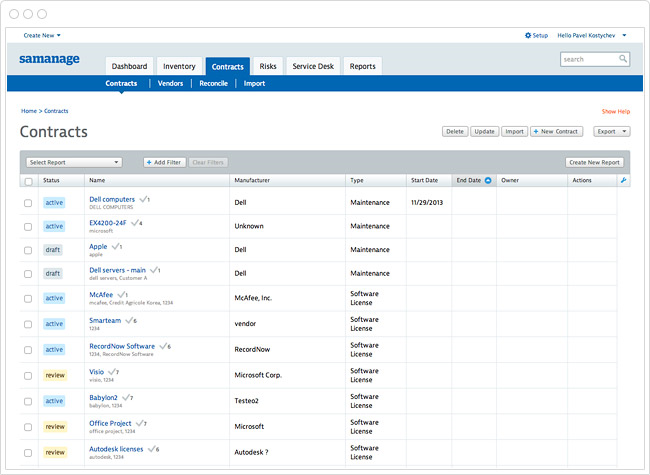
\includegraphics[scale=0.6]{Images/samanage/Contract_license.png}
\caption{Gestione di contratti e licenze}
\label{sd-samanage-contract-license-img}
\end{figure}

Permette inoltre di tenere traccia dei pagamenti effettuati a seguito di rinnovi, e di impostare dei promemoria vicino alle date di scadenza delle licenze/contratti affinché sia possibile rinnovarli senza alcuna perdita di servizio.

\subsection[Gestione della Knowledge Base e del portale self-service]{gestione della knowledge base del portale self-service}
\label{sd-samanage-knowledge-base}
Il \english{software} consente di conservare in un unico posto logico (vedi figura \ref{sd-samanage-knowledge-base-img-1}) tutte le \english{best practices} e le soluzioni a richieste comuni.

\begin{figure}[htbp]
\centering
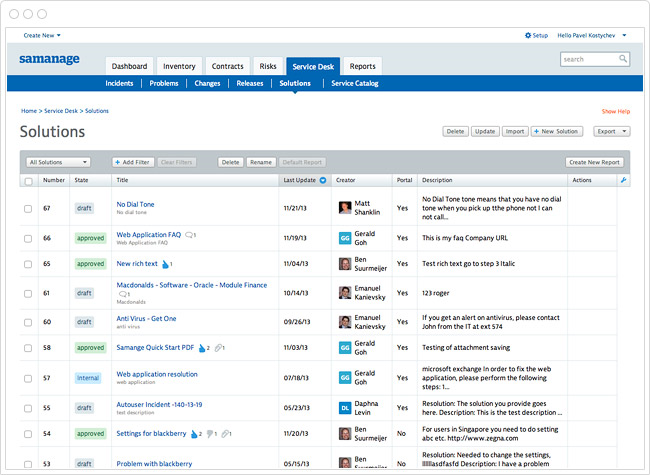
\includegraphics[scale=0.6]{Images/samanage/Knowledge_base.png}
\caption{Gestione della \ac{Knowledge-Base} per lo staff tecnico}
\label{sd-samanage-knowledge-base-img-1}
\end{figure}

Utilizzare il sistema integrato di gestione della \ac{Knowledge-Base} consente di ridurre i tempi di risoluzione dei problemi, e servire da piattaforma di condivisione della conoscenza, perché accessibile a tutti gli utenti dei servizi (vedi figura \ref{sd-samanage-knowledge-base-img-2}). 

Questo portale è il portale ``\english{self-service}'' in cui gli utenti posso accedere alle soluzioni a problemi comuni.

\begin{figure}[htbp]
\centering
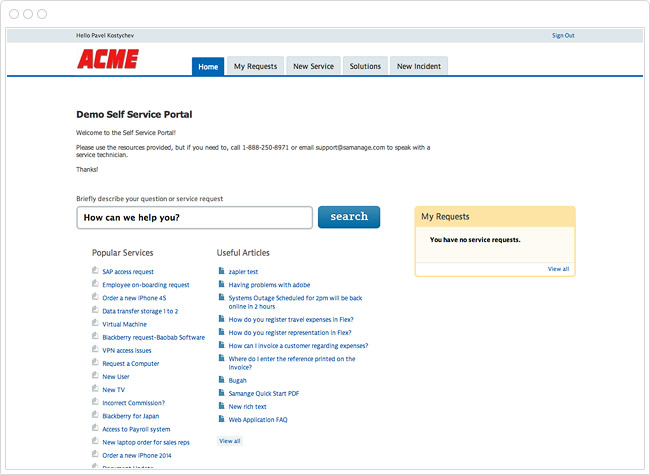
\includegraphics[scale=0.6]{Images/samanage/Knowledge_base_self_service.png}
\caption{Accesso alla \ac{Knowledge-Base} per gli utenti}
\label{sd-samanage-knowledge-base-img-2}
\end{figure}

Questo aumenta l'efficienza di supporto e aumenta la consapevolezza effettiva della conoscenza \acs{Information-Technology} in tutto l'istituto.

\subsection[Gestione ed analisi dei report]{gestione ed analisi dei report}
\label{sd-samanage-report-management}
Il \english{software} fornisce un robusto e flessibile sistema di gestione dei report e dei \english{feedback} degli utenti, che consente di mantenere sempre sotto controllo le attività svolte dallo staff tecnico.

\begin{figure}[htbp]
\centering
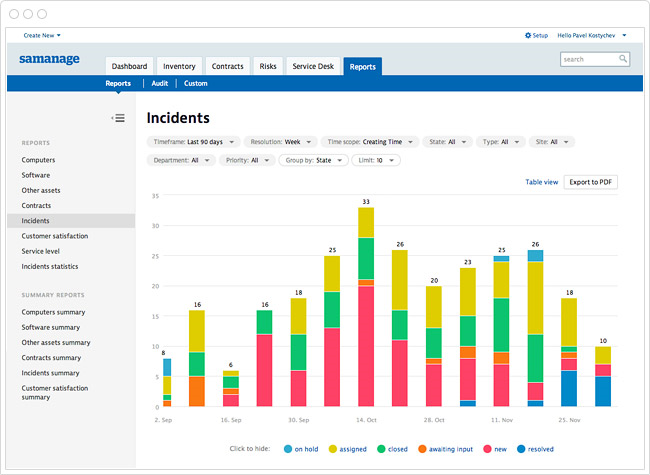
\includegraphics[scale=0.6]{Images/samanage/Report_management.png}
\caption{Gestione ed analisi di report}
\label{sd-samanage-report-management-img}
\end{figure}

E' possibile filtrare ed analizzare i dati, scoprire importanti \english{patterns} e \english{trends} che possono impattare le \english{performance} dell'ambiente \acs{Information-Technology} (vedi figura \ref{sd-samanage-report-management-img}).

\subsection[Integrazione con Active Directory]{integrazione con Active Directory}
\label{sd-samanage-active-directory}
\acf{Active-Directory} è uno dei più popolari metodi per gestire i \english{files} degli utenti, i permessi e le informazioni di contatto all'interno di un dominio \english{Microsoft Windows}.

Samanage rende semplice la sincronizzazione dell'\ac{Active-Directory} dell'istituto consentendo di controllarlo da un unico posto centralizzato.

\subsection[Gestione degli assets]{gestione degli assets}
\label{sd-samanage-assets-management}
Con il modulo di \acs{Information-Technology} \ac{Asset-Management} lo staff tecnico è in grado di controllare più agevolmente lo scenario tecnologico presente nell'istituto.

Questo modulo offre potenti strumenti e funzionalità che comprendono un sistema continuo per tenere traccia dell'inventario \english{hardware} e \english{software} dell'istituto, compresi i \acs{Personal-Computer}, server, \english{laptop}, dispositivi \english{mobile}, dispositivi di rete e qualsiasi altro \english{asset} tecnologico presente. In figura \ref{sd-samanage-asset-management-img} è possibile vedere la schermata che permette la gestione degli \english{asset}.

\begin{figure}[htbp]
\centering
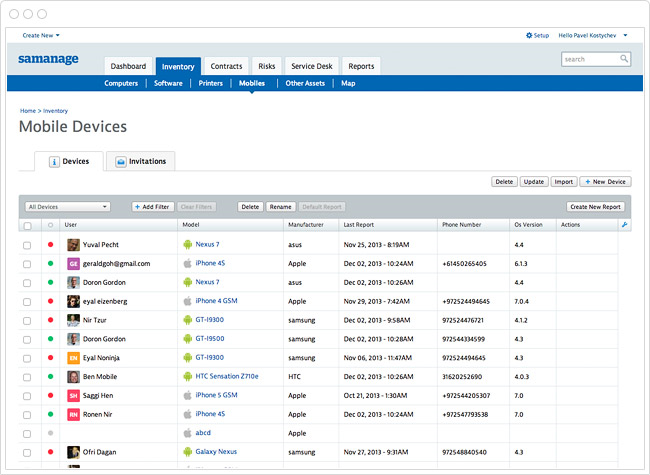
\includegraphics[scale=0.6]{Images/samanage/Asset_management.png}
\caption{Gestione degli \english{asset}}
\label{sd-samanage-asset-management-img}
\end{figure}

Il modulo aiuta inoltre a garantire la conformità del \english{software}, aumentare la sicurezza e ridurre al minimo i costi attraverso una soluzione di semplice utilizzo per la gestione degli \english{asset}.

\subsection[Gestione di possibili anomalie]{gestione di possibili anomalie}
\label{sd-risk-management}
La gestione del rischio \acs{Information-Technology} può e deve essere considerato come un componente primario di un più ampio scenario di gestione del rischio aziendale, e quindi è desiderabile investire in un sistema di controllo efficace.

La soluzione \english{software} proposta consente di gestire le situazioni di rischio aiutando lo staff tecnico a concentrarsi sulle aree che richiedo maggior attenzione nell'ambiente \acs{Information-Technology}.

\begin{figure}[htbp]
\centering
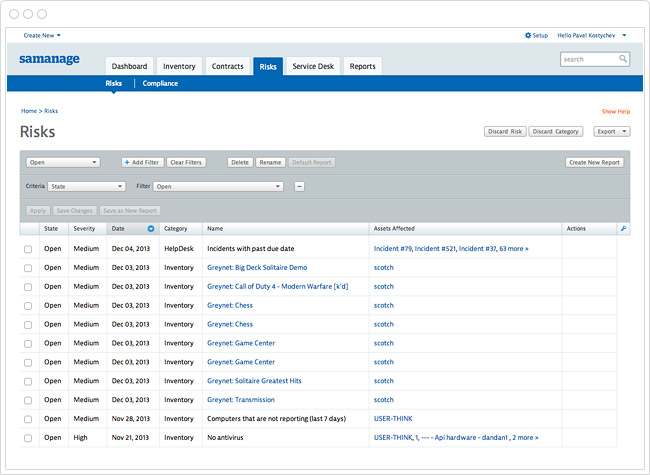
\includegraphics[scale=0.6]{Images/samanage/Risk_management.png}
\caption{Schermata che consente di tenere le problematiche sotto controllo}
\label{sd-samanage-risk-management-img}
\end{figure}

Esso include un motore di rilevamento del rischio che analizza costantemente i dati memorizzati nella sua banca dati (come per esempio l'inventario delle attività o richieste al \english{Service Desk}) e cerca modelli problematici. Se ne dovesse rilevare alcuni saranno in automatico aperte delle notifiche (vedi figura \ref{sd-samanage-risk-management-img}) che possono essere viste dal personale del \english{Service Desk}.

\subsection[Gestione di problemi e cambiamenti]{gestione di problemi e cambiamenti}
\label{sd-problem-change-management}
La soluzione \english{software} proposta fornisce strumenti per la gestione e l'approvazione delle modifiche ai \ac{Configuration-Item} presenti nell'ambiente \acs{Information-Technology}.

Questo consente di trovare soluzioni permanenti ai problemi e prevenire gli incidenti ripetuti che causano interruzioni del servizio.

Attraverso gli strumenti di approvazione delle modifiche possiamo garantire che le modifiche effettuate dal processo di \ac{Change-Management} siano in linea con la strategia aziendale complessiva prima della loro messa in produzione.

\subsection[Gestione del service catalogue]{gestione del service catalogue}
\label{sd-service-catalogue-management}
Samanage permette la gestione di un \english{Service Catalogue} in linea con le \english{best practice} \ac{Information-Technology-Infrastructure-Library}.

\begin{figure}[htbp]
\centering
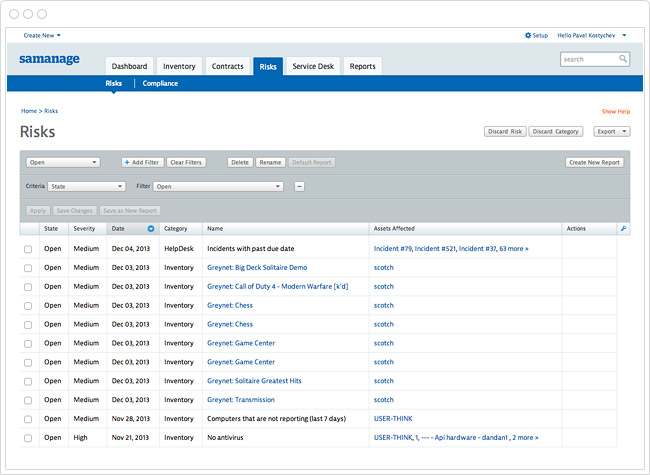
\includegraphics[scale=0.6]{Images/samanage/Risk_management.png}
\caption{Schermata che consente di tenere le problematiche sotto controllo}
\label{sd-samanage-service-catalogue-img}
\end{figure}

Sarà possibile definire e pubblicare, all'interno del portale (vedi figura \ref{sd-samanage-service-catalogue-img}), i servizi disponibili con le relativi soluzioni per gestire al meglio i carichi di lavoro.

Questo incoraggia gli utenti all'uso del portale \english{self-service} consentendo quindi loro di effettuare delle richieste di servizio da un elenco prestabilito, agevolando cosi il lavoro dello staff di \english{Service Desk}.

\subsection[Gestione dei documenti di SLM]{gestione dei documenti di SLM}
\label{sd-sla-management}
Gli accordi sui livelli di servizio offerti sono una parte importante della gestione del dipartimento \acs{Information-Technology}.

Gli \ac{Service-Level-Agreement} definiscono come viene effettuata la misura delle \english{performance}, la gestione dei problemi, le garanzie, i tempi di risposta ecc. Con adeguati obiettivi di \ac{Service-Level-Agreement} il dipartimento sarà in grado di garantire ottimi livelli di servizio ed assicurare che il servizio offerto rispetti gli accordi.

\begin{figure}[htbp]
\centering
\includegraphics[scale=0.6]{Images/samanage/Service_level_management.png}
\caption{Schermata che consente di tracciare gli \ac{Service-Level-Management}}
\label{sd-samanage-service-level-management-img}
\end{figure}

La soluzione proposta consente di gestire in unico posto (vedi figura \ref{sd-samanage-service-level-management-img}) tutti i documenti e tracciarne le eventuali modifiche affinché nulla vada perso o sia lasciato al caso.






























\clearpage
\printGlossary{TRUE}

\end{document}